\section{AutoMArch}
AutoMArch is capable of creating multi-threaded in-order designs of any number of threads and any number of pipeline stages that is functionally equivalent to n-copies of the input base functional datapath, where n is the number of threads. The functionality of the input base datapath is defined by its input output behavior and its next state update behavior. Two designs are defined as functionally equivalent if given the same starting architectural state and sequence of inputs, the two designs transition to the same ending architectural state and produce the same sequence of outputs. Architectural state elements are defined as the state elements present in the input base functional datapath. AutoMArch always preserves the state elements present in the input base functional datapath, but may add additional state elements such as pipeline registers that are not considered architectural state. AutoMArch takes an input base functional datapath specified in Scalpel and outputs the multi-threaded in-order design as a Chisel source file, which can be feed into various simulation, FPGA, and ASIC flows.

\subsection{Input Datapath Restrictions}
\label{section:InputRestrictions}
The input base functional datapath can be an arbitrary FSM specified in Scalpel with the following restrictions:

{\bf (1)} The input FSM must communicate to the outside world through ready/valid ports  

{\bf (2)} The designer cannot use input valid or output ready signals as inputs to any part of their circuit

{\bf (3)} Any functional units that may take more than one clock cycle to return responses(caches, multipliers, dividers, etc) must be accessed through the Variable Latency Unit Interface discussed below.

Condition {\bf (1)} is necessary because the transformed design will have different input to output latency than the original design depending on what stages the input and output ports are placed in the pipeline. Additionally, some pipeline stages may contain bubbles or be stalled and it would be incorrect to receive inputs or produces outputs under these conditions. Thus by enforcing that only ready/valid IO ports are used, correct IO behavior can be defined by only the sequence of valid inputs tokens accepted and sequence of valid outputs tokens produced, without any restriction on the exact timing of when the input tokens are accepted and output tokens are produced.

\subsubsection{IO Semantics}
When input ready or output valid is driven high by the input FSM, this implicity signals to the tool that the input FSM requires the use of the input or output port on the current state update. Thus, the tool generates logic that examines the input ready or output valid and stalls the pipeline if the corresponding input valid or output ready is not driven high by external modules. The designer should design the input FSM so that input readies and output valids are only driven high when absolutely necessary to avoid unnecessary stalling the automatically multi-threaded and pipelined version of the circuit.

\begin{figure}
	\centering
    \resizebox{\columnwidth}{!}{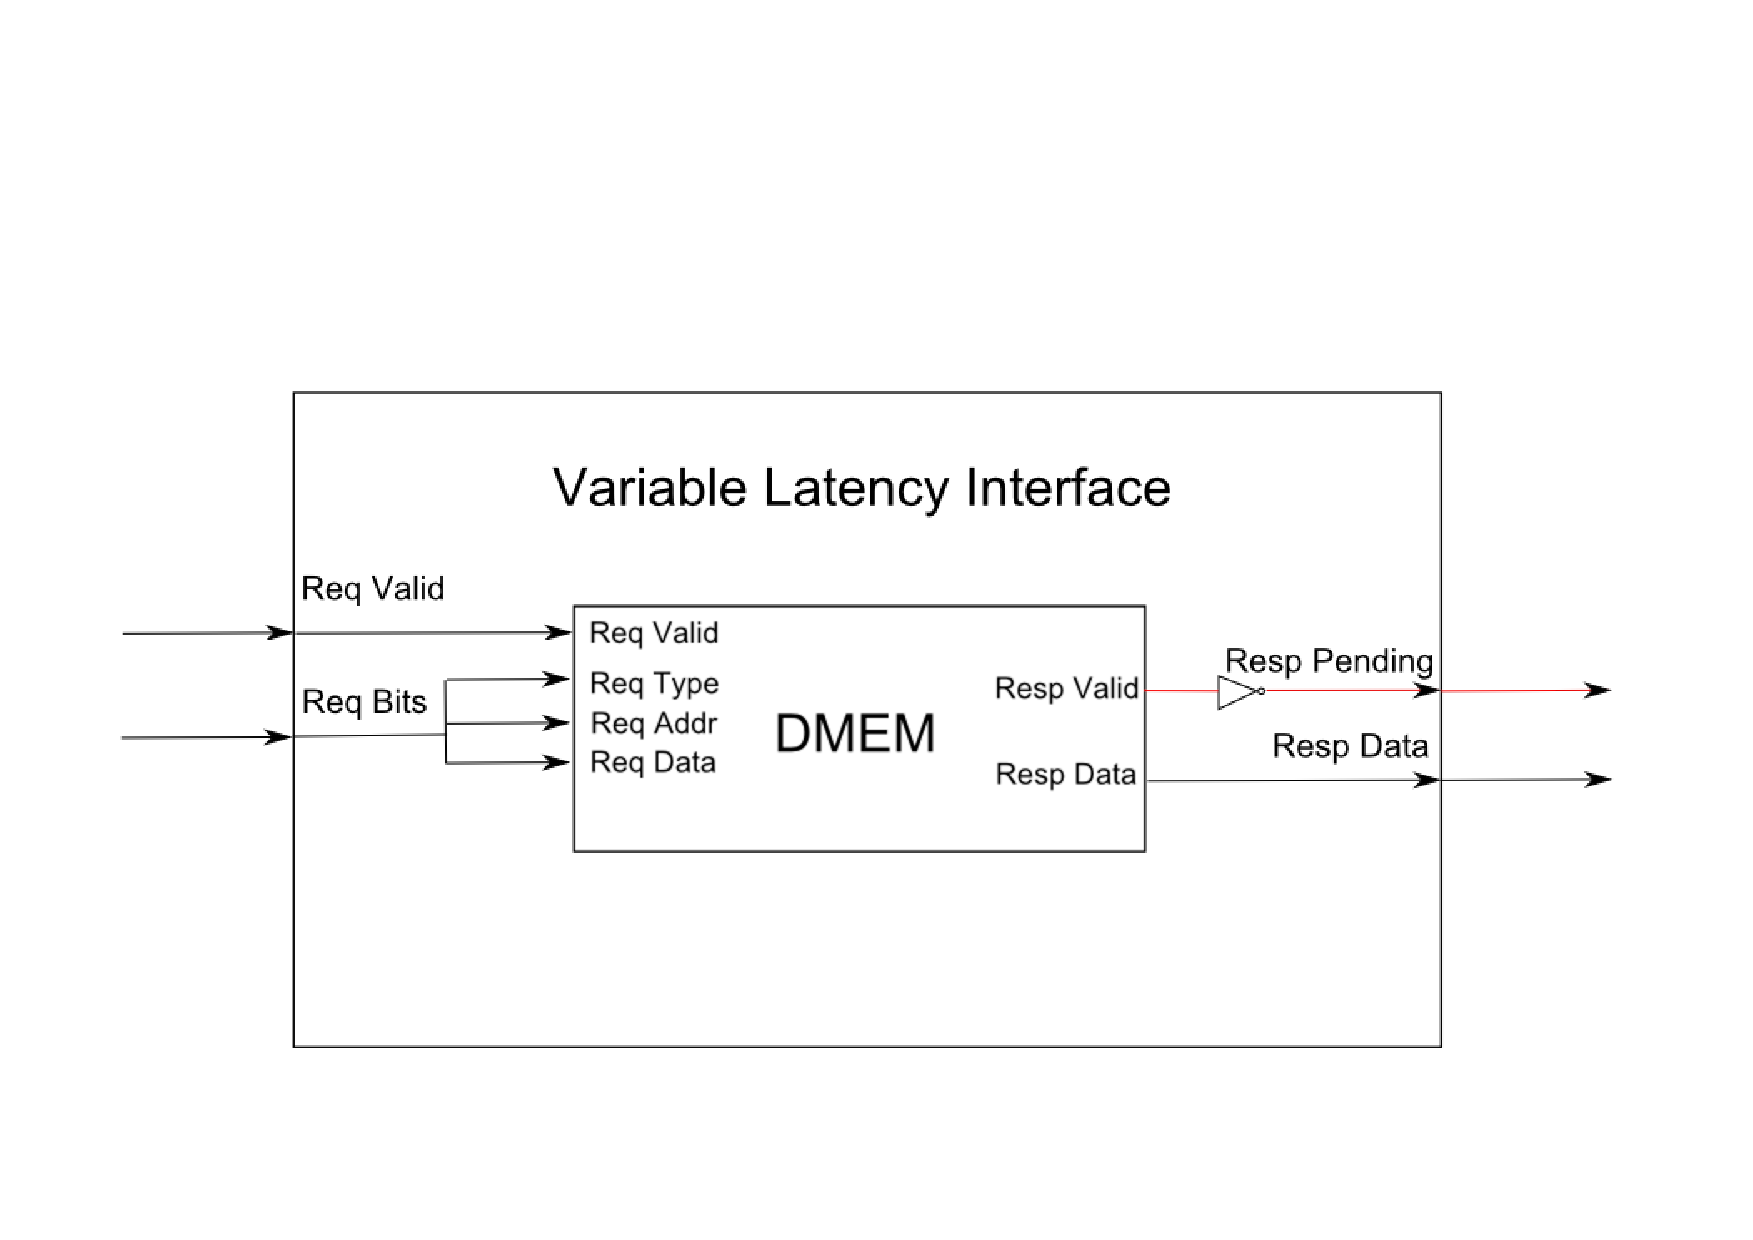
\includegraphics{figures/TransactionalInterface}}
    \caption{{\bf Single Thread View of Variable Latency Unit Interface} Black wire are user facing IO, red wires are tool facing IO}
	\label{fig:VarLatIO}
\end{figure}

\subsubsection{Variable Latency Unit Interface}
In order to accomodate caches and long latency arithmetic units in the minimal FSM specification that is not allowed to have any optimization or control logic implemented, the tool provides the Variable Latency Unit Interface. The designer should access any caches or long latency arithmetic units through a Variable Latency Unit Interface and treat that Variable Latency Unit Interface like a piece of combinational logic in the input FSM specification. IE the designer should not use the Resp Pending port of the Variable Latency Unit Interface to drive any part of their circuit and should pretend that the Variable Latency Unit Interface always gives a valid response immediately. The tool will automatically generate control logic that deals with the Variable Latency Unit Interface not immediately outputting a valid response.

\subsection{Conventions}
\label{section:conventions}
{\bf State Element Partitioning}
State elements in the input FSM will be considered as multiple circuit components. For singular registers, the read output is considered a separate component from the write data and write enable inputs and will be referred to as the register's read port. The write data and write enable input is considered together as a single circuit component and will be referred to as the register's write port. For memories, which could be either an array of registers or a SRAM block, each read port and each write port is considered a separate component. 

This partitioning of the state elements into separate read and write ports make it easier for AutoMArch to analyze the input datapath because it allows the datapath to viewed as a acyclic circuit component graph in which data flows from the state element read ports and input pins through combinational logic nodes into the state element write ports and and output pins.

{\bf Pipeline Terminology}
Traditionally, in order pipelining is discussed with regards to processors or stateless combinational units. Pipelining stateless combinational units is trivial as there are no inter-pipeline stage dependencies. When pipelining processors, we consider the dependencies between each instruction flowing down the pipeline when creating pipeline control logic. However, pipelining as discussed in this thesis can be applied to arbitrary finite state machines. In this context, it does not make sense to talk about instruction to instruction dependencies as we are not only dealing with arbitrary FSMs. Instead, we will consider there to be a series of next state updates flowing down the pipeline. When constructing pipeline control logic, we will consider dependencies between each next state update flowing down the pipeline.

\subsection{Automatic Pipelining}
\subsubsection{Pipelining Options}
\label{section:pipelineOptions}
First the designer must select the number of pipeline stages the optimized design should have. This is the minimum specification needed. If no additional specification is provided, the tool will automatically place all of the pipeline registers and default to generating an inorder pipeline that resolves all pipeline hazards by interlock.

{\bf Pipeline Stage Placement}
By default, the tool places all of the architectural state element read ports in the first pipeline stage and the architectural state element write ports along with the output ready/valid ports in the last pipeline stage. The tool then automatically place the rest of the circuit components in a pipeline stage that minimizes the critical path delay.

If this default placement is not suitable, the designer is given the option to manually place specific circuit components. For example, in a RISC processor design, the PC register write port should be placed as early as possible in the pipeline to minimize branch penalty. The designer does this by annotating circuit components with the desired stage number in the RTL source file of the base functional datapath. Then when the tool does the automatic placement of the circuit components, it will first place the user annotated components in their specified pipeline stage before it automatically places the rest of the unannotated circuit components. 

Thus, the designer has the flexibility to manually place none, some, or all of the circuit components in the base functional datapath. The designer can initially let to the tool place all of the circuit components and gradually manually place components as performance issues are discovered.

{\bf Pipeline Hazard Resolution}
In the traditional framework of inorder processor pipeline design, there are three types of hazards - data hazards, control hazards, and structural hazards. Only data hazards need to be dealt with by the tool. Data hazards arise when the next state update in pipeline stage X reads a state element R that could be written by a next state update in pipeline stage Y, where Y {\tt >} X, but Y {\tt <=} the stage of the R's write port. This situation would make the next state update in pipeline stage X use stale read data and result in a non functionally correct design. In traditional pipelined processors, control hazards arise when the next PC information is not available soon enough for branch and jump instructions. This is really just a data hazard on the PC register and does not need to be considered separately. Likewise, in traditional pipelined processors structural hazards arise when instructions in different stages of the pipeline need to write to the register file at the same time, but there is only one register file write port. This cannot happen in AFDO because the input base functional datapath does not have multiple pipeline stages and the tool will not generate logic to have instructions at different pipeline stages write to the same architectural state element write port.

There are three common ways to resolve data hazards - interlocking, bypassing, and speculation. Each option has different performance and area characteristics. The tool generates logic that implements interlocking by default. The designer may choose bypassing or speculation on a read port by read port basis by annotating the particular architectural state element read port they want to be bypassed or speculated in the base functional datapath RTL source. Details of each hazard resolution option will be discussed in \ref{section:logicGen}

\subsubsection{Circuit Node Graph Creation}
Because AutoMArch uses Scalpel to specify the input base functional datapath, it does not need to do any additional work to create a node graph data structure representing the input base datapath. Scalpel's internal data structure already uses a node graph to represent the design. All IO pins, wire, logic gates, and state element read and write ports are represented as individual nodes and all nodes maintain a list of its inputs and a list of its consumers. This node graph is convinient for AutoMArch to use directly because it follows the conventions in \ref{section:conventions} as it uses separate graph nodes to represent every state element's read and write ports and by extension has a acyclic node graph. AutoMArch modifies Scalpel's internal node graph data structure directly and uses Scalpel's buildt in elaboration methods to produce the Chisel source file that represents the final multi-threaded and pipelined design.

\subsubsection{Pipeline Register Placement}
The automatic pipelining tool first creates a legal placement of pipeline registers and then creates a optimized placement by balancing the critical path delay in each stage. The automatic placement process preserves the user specified pipeline stage of user annotated base datapath components.


{\bf Pipeline Legality}

For a pipeline register placement to be legal, it must satisfy the following conditions:

{\bf (1)} Every combinational logic node has all input signal with the same stage number.  

{\bf (2)} The stage number of every combinational logic node's output signal is equal to the shared stage number of its input signals.

{\bf (3)} There are two ways to determine the stage number of a node. One way is to trace through the node's inputs to a pipeline register and set the stage number of the node equal to the stage number of that pipeline register. Another way is to trace through the node’s consumers to a pipeline register and set the stage number of the node equal to the stage number of that pipeline register {\tt -}  1. For all nodes in the graph, the stage number of the node obtained through both methods must be the same.

{\bf (4)} All the read ports of a state element must have the same stage number and all the write ports of a state element must have the same stage number. The stage number of a state element's read port(s) must {\tt <=} that state element's write port(s).

{\bf (5)} All of the user facing IO pins of a Variable Latency Unit Interface must have the same pipline stage number, as the designer treats a Variable Latency Unit as a combinational logic unit.

{\bf (6)} Every input ready/valid IO must have a stage number <= the minimum stage number of every output ready/valid IO. (inputs must be placed before outputs)

It is possible that the designer manually annotates the base datapath in such a way that no legal pipeline register placement can be produced without changing the stage of the user specified components. If this is the case, an error is triggered.


{\bf Obtaining a Initial Legal Placement}

To make pipeline register placement easier, the tool creates a slightly modified node graph to represent the input base datapath. In this modified node graph, all of the read ports of a state element are merged into one node and all of the write ports of a state element are merged into one node, in order to maintain pipeline legality condition {\bf (4)}. Then, all of the user facing IO pins of a Variable Latency Unit Interface are merged into one node in order to maintain pipeline legality condition {\bf (5)}. Then all of the pins associated with a ready/valid port are merged into a single node. Additionally, a node representing a wire is inserted between all combinational logic nodes in the original design. This ensures that a pipeline boundary never has to fall across a combinational logic node, which would be difficult to reconcile with the notion of Pipeline Legality discussed above. All other aspects of the Scalpel node graph remain the same.

In this node graph, the register readports are source nodes(which have no inputs) and all architectural state element write ports and output ready/valid ports are sink nodes(which have no consumers). All nodes in the input base datapath can be reached through the source nodes' consumer pointers, with the execption of nodes driven only by constants, which don't need to be considered in the pipeline register placement process. All nodes in the input base datapath can be reached through the sink nodes' input pointers. The tool produces the initial legal pipeline placement by propagating stage numbers out from the source nodes to their consumers and the sink nodes to their inputs in a pseudo breadth-first-search (BFS) manner. When two propagation frontiers with different stage numbers meet at the same node, propagation down that path stops and pipeline registers are inserted at that node. The source and sink nodes are guaranteed to have pipeline stage numbers at the beginning of the process, whether through user annotation or through the defaults mentioned in \ref{section:pipelineOptions}

We must maintain the following conditions during the pipeline stage propagation process:

{\bf (1)} Adjust the propagation rates of each propagation frontier so that two different propagation frontiers never meet at a combinational logic node and always meets at a wire node, because it does not make sense to split a combinational logic node in half with a pipeline register.

{\bf (2)}  The stage number propagated to a combinational logic node with multiple inputs must be the maximum of the stage numbers of all of its inputs. If this was not maintained, we would have some inputs of the combinational logic node have a greater stage number than the stage number of the output of the combinational node, which violates 2nd condition of Pipeline Legality. This also means that we cannot propagate to a Chisel node with multiple inputs from the input side until all of its inputs have been propagated to.

{\bf (3)} The stage number propagated to a combinational logic node with multiple consumers must be the minimum of the stage numbers of all of its consumers. If this was not maintained, we would have some consumers of the combinational logic node have a smaller stage number than the stage number of the output of the combinational node, which cause that consumer to violate the 3rd condition of Pipeline Legality. This also means that we cannot propagate to a Chisel node with multiple consumers from the consumer side until all of its consumers have been propagated to.


{\bf Obtaining an Optimal Placement}

After a legal pipeline register placement is obtained, the tool automatically optimizes the pipeline register placement with regards to critical path delay by balancing out the critical path length in each pipeline stage. 

It does this by first assigning a delay value for each node in the node graph. In the current implementation, a naive assignment is used. All combinational logic nodes are assigned a delay of 1.0 and all wires are assigned a delay of 0.0. Memory read ports as well as Variable Latency Units are also assigned a delay of 1.0. A more sophisticated assignment based on the delay data collected from ASIC tools could be used, but this naive assignment is mostly sufficient because VLSI retiming can be applied on top of the pipeline register placement performed by the tool. Thus, the pipeline register placement optimization only has to be approximately correct to produce good critical path delay once the design is pushed out through the ASIC design flow. Additionally, real ASIC delay characteristics cannot be fully captured by a static assignment of delay values to each node because they are highly dependent on gate level optimizations performed by the ASIC tools, which varies per design, as well as wire delays, which are dependent the layout of the circuit. So putting too much effort into assigning highly accurate delay values to nodes is futile anyways. 

Then, the tool uses the following pressure based algorithm to move the pipeline stage boundaries:

{\bf (1)} The tool finds the critical path in each pipeline stage and calculates their delays.

{\bf (2)} On each pipeline stage boundary, the side with the longer critical path delay "pushes" the boundary towards the other side. This "push" is accomplished by taking the end node from the critical path on the side with the longer critical path delay and moving it across the pipeline boundary.

{\bf (3)} Repeat until the maximum critical path of all the stages stops decreasing.

\subsubsection{Data Hazard Resolution Option Details}
\label{section:logicGen}
Data hazard resolution options are selected on a read port per read port basis. Every read port of every architectural state element can have a different data hazard resolution option. By default, data hazards on every read port is resolved by interlocking and the designer can annotate the read ports whose data hazards they want to be resolved by bypassing or speculation.

{\bf Interlocking}

Interlocking is the simplest way to resolve data hazards. When the next state update at stage X has the possiblity of using stale read data due to a next state update at stage y {\tt >} x writing to an architectural state element being read by the next state update at stage X, we simply stall the pipeline at stage X and inject bubbles into stage X + 1 until the next state update at stage y flows down the pipeline and finishes writing to the architectural state element. Interlocking has the lowest cost in terms of area and cycle time, but has the highest cost in terms of performance because it inserts bubbles into the pipeline whenever a data hazard occurs.

{\bf Bypassing}

Bypassing allows data hazards to be resolved with fewer bubbles inserted into the pipeline if the write data and write enable signal of the contested architectural state element is earlier than the stage of the write port by inserting muxing the read data pin of the read port with the write data signal as soon as it is available. If the write data and write enable signals are available in the stage immediately after the read port, no bubbles need to be inserted at all. If the write data and write enable signals are only available at the stage of the write port, then bypassing does not produce fewer bubbles than interlocking. Compared to interlocking, bypassing has higher cost in terms of area and cycle time due to the bypass network, but has lower cost in performance because inserts fewer bubbles into the pipeline.

In order to select bypassing as the data hazard resolution option, the designer simply annotates the desired read port as bypassed in the RTL source file of the base functional datapath.

{\bf Speculation}

For certain architectural state elements such as the PC register in RISC processors, interlocking is not acceptable because of the performance penalty and bypassing does not help because the write data signal of the PC register's write port is not immediately available. In these cases, it is desirable to speculate on the next read value of the architectural state element and then kill next state updates present in the pipeline between the stage of the read port and the stage of state element write port, including the next state update present in the stage of the read port, if the speculated value is determined to be incorrect later.

Control logic generation for arbitrary speculation is very complex, so the tool places the following restrictions on what kind of speculation maybe performed:

{\bf (1)} Only the read ports of registers maybe speculated upon.

{\bf (2)} There may only be one speculated register read port per pipeline stage.

{\bf (3)} Assuming the stage of a speculated read port is stage X and the stage of the corresponding write port is stage Y, there may not be IO ports, Variable Latency Units, architectural state element write ports, and other speculated read ports present in the stages between stage X and stage Y, inclusive of stage X.

The user specifies that a register read port should be speculated upon in by annotating the desired read port as speculated in the RTL source file of the base functional datapath. The user creats a speculative clone of the register associated with the read port speculated upon and creates the update logic for that speculative clone register in the RTL source of the base funtional datapath. Then the user uses some annotations to label this clone register as the speculative clone of the original register. The tool will generate control logic that muxes the read data port of the original register with the read data port of the speculative clone register. The read data from the speculative clone register will be choosen except on the clock cycle immediate after a mispredict. During that cycle, the data held in the speculative clone register is synced with the correct data in the original register.

\subsubsection{Pipeline Control Logic Generation}
After the tool places the pipeline registers, it then automatically generates the pipeline control logic that keeps the functional behavior of the pipelined data path the same as the functional behavior of the base input circuit. The pipeline control logic will need to deal with both the availability of valid tokens at the ready/valid IO ports as well as the data hazards introduced by pipelining. I will first present the scheme necessary to generate control logic that deals with the availability of IO ports and handles all data hazards through interlocking. Then I will present the control logic needed for bypassing and speculation as modifications on top of the basic interlocking scheme.

The following signals are generated in the basic interlocking scheme:

{\bf IOBusy Signals}

An IO port is considered busy if the input ready/output valid signal is driven high, which implicitly signals that the data from this port is needed to be consumed/produced, and the input valid/output ready signal is driven low by an outside module, which indicates that the port is not available.


{\bf VarLatIOBusy Signals}

A Variable Latency Unit is busy if its RespPending port is driven high.


{\bf RAW Hazard Signals}

A read port belonging to stage X is considered to have a RAW hazard if a pipeline stage Y is valid, has the same thread ID as stage X, and contains a transaction that could write to any write port that belongs to the same state element as the read port.


{\bf Valid Signals}

The tool generates a valid signal for each pipeline stage. Each pipeline stage is currently valid if the previous pipline stage was valid on the last clock cycle, no state element read ports in this pipeline stage has a RAW hazard, no IO port in this stage is busy, and there are no kill signals triggered in this stage. The input ready signals, output valid signals, Variable Latency Unit Interface Req Valid signals, and state element write enable signal are masked with the valid signal for the pipeline stage they belong in.


{\bf Stall Signals}

The tool generates a stall signal for each pipeline stage. When a pipeline stage is stalled, the contents of that pipeline stage does not progress into the next pipeline stage. The boolean equation for stage X's stall signal = stage X + 1 is stalled OR (stage X was valid last cycle AND (a read port in stage X+1 has a RAW hazard OR a IO port in stage X+1 is busy)). The input ready signals, output valid signals, Variable Latency Unit Interface Req Valid signals, and state element write enable signal are masked with the valid signal for the pipeline stage they belong in. 


\subsubsection{Differences From VLSI Retiming}
The automatic pipelining ability of AutoMArch appears to be similar to well known VLSI Retiming methods, but it is much more powerful. VLSI Retiming methods are only capable of adding pipeline stages to purely combinational datapath or moving registers around in a manually pipelined sequential datapath. It is not capable of adding pipeline stages to an unpipelined sequential datapath and the way it can move registers around in a manually pipelined sequential datapath is contrained by the placement of the manually constructed pipeline control logic. AutoMArch is capable of adding pipeline stages to arbitrary sequential datapaths as long as they follow the restrictions in \ref{section:InputRestrictions}. Additionally, AutoMArch has full freedom to place the pipeline registers in sequential datapaths because it can generate the correct pipeline control logic for any legal pipeline register placement.

\subsubsection{Example Application}

\subsection{Automatic Multi-threading}
%present automatic multi-threading as a modification of the automatic pipelining scheme
\subsubsection{Multi-threading Options and Specification}
\subsubsection{Pipeline Control Logic Generation}
\subsubsection{Example Application}
